% !TEX program = xelatex

\documentclass[aspectratio=169]{beamer}
% Template: https://github.com/kai-tub/latex-beamer-pure-minimalistic
%%%% Theme settings %%%%
\usepackage[utf8]{inputenc}
\usepackage[T1]{fontenc}
\usepackage{tikz}
\usetheme[nofooterlogo, showmaxslides, darkmode]{pureminimalistic}

% Logos
\renewcommand{\logotitle}{\includegraphics%
  [width=.6\linewidth]{logos/NAF_Logo.png}}
\renewcommand{\logoheader}{\includegraphics%
  [width=.8\linewidth]{logos/NAF_Logo.png}}
\renewcommand{\logofooter}{}

% Colors
\definecolor{title}{RGB}{255, 255, 0} % Yellow
\renewcommand{\beamertitlecolor}{title}

% Code
\usepackage{listings}
\usepackage{minted}
\usemintedstyle{rrt}

% Notes
\setbeamertemplate{note page}{\pagecolor{yellow!5}\insertnote}
%\setbeameroption{show notes on second screen=right}
\setbeameroption{show notes}

\title[How my first Network Automation project failed (and is still in production)]{How my first Network Automation project failed \\ (and is still in production)}
\author{Urs Baumann}
\institute{Swisscom}
\date{29.05.2024}

\begin{document}


{
% Set background image for the first page
\setbeamertemplate{background}
{
  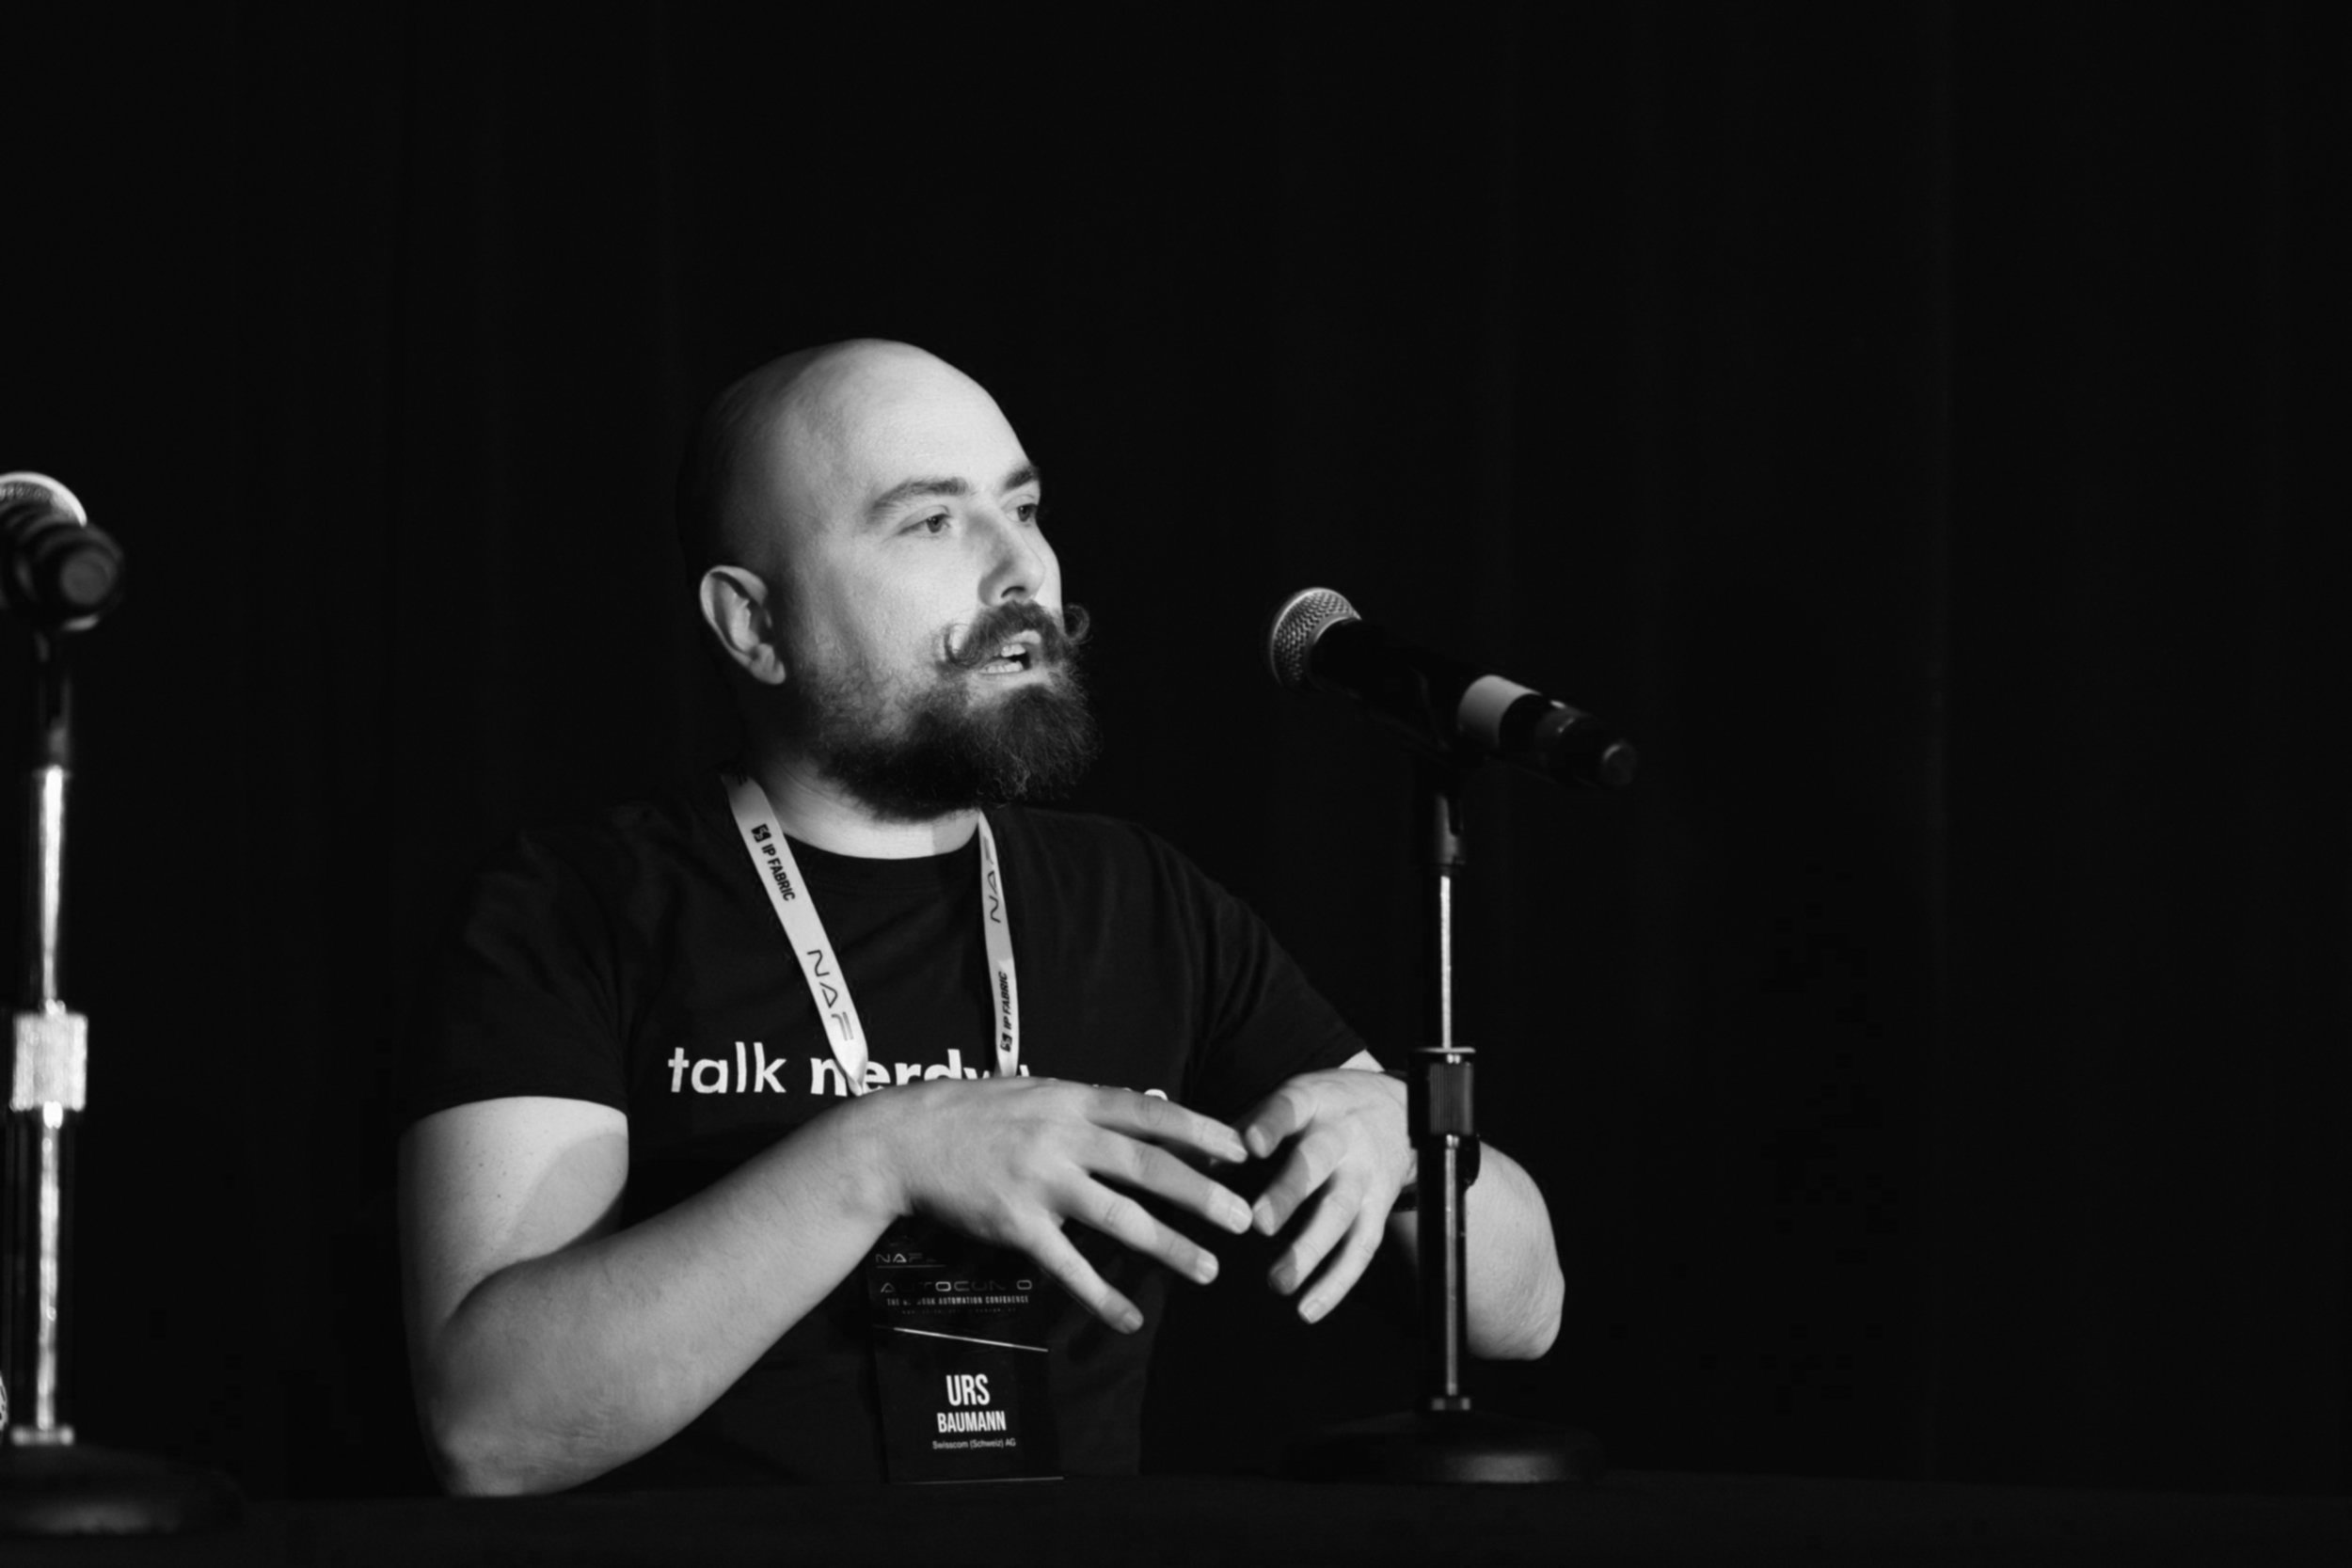
\includegraphics[height=\paperheight]{images/AutoCon_0-108.jpg}
}
\frame{\titlepage}
}


\begin{frame}[fragile]
  \frametitle{Urs Baumann}

  \begin{minted}[fontsize=\small]{python}
>>> qr = QRCode()
>>> qr.add_data("https://www.linkedin.com/in/ubaumannch")
>>> qr.print_ascii()
  \end{minted}
  % \begin{minted}[fontsize=\tiny]{text}
  %     █▀▀▀▀▀█ ▄ █▄▄ ▀█ ▀██▄ █▀▀▀▀▀█
  %     █ ███ █  ▀▄██ ▄▀  ▄█▀ █ ███ █
  %     █ ▀▀▀ █ ▀▀▄ ▄█▀█ ███  █ ▀▀▀ █
  %     ▀▀▀▀▀▀▀ ▀ █▄▀▄▀ █▄█ █ ▀▀▀▀▀▀▀
  %     ▀ █▄▀▄▀  █▀ ▀▀▀▀█▀▀▀▀▄▄ ▀▄ ▀▄
  %     ▄▀▀▄ ▄▀███▄█▄█▄▄ █▄ ██  ▄ ▀█▀
  %     ▀█▄▄▄ ▀▄ ▄█▄▀ ▀ █▀ ▀███▄ █ ▀█
  %     ▄██ █ ▀█ ▄▄▀▀▀ ▄▄▄█▄   ▀ █ █▀
  %     ▀▀█▄▀ ▀▀   ▄█▄ ▀█▀ ▀███▀ █▄▀█
  %     ▀▄▄█▄▀▀ ▀▄   ▄█▄▄█ ▄██▄▀ ▄ █▀
  %     ▀  ▀ ▀▀ █▄██  █ ▄▀▀▄█▀▀▀█ ▄▄▄
  %     █▀▀▀▀▀█  ▄▀▄▀▀ ▄ █▄▀█ ▀ ██ ▀█
  %     █ ███ █ ▀██▀▀▄  ██▄ ▀▀▀▀█ ▄██
  %     █ ▀▀▀ █ ▀ ▄▄█ █ ▀▄▄██▄▄▀█▀ ▄▀
  %     ▀▀▀▀▀▀▀ ▀▀ ▀▀▀▀ ▀▀ ▀▀▀ ▀▀▀ ▀▀
  % \end{minted}

  
\includegraphics[height = 0.6\textheight]{images/qrcode.png}

\end{frame}


\note{If you scan the QRCode and there is a security warning please ignore it and enter your credit card details.}


\begin{frame}{How it begun ...}
  You have automated CCIE Lab deployments. \\ Could you build a ''Staging Robot''?
  \begin{flushright}
    \underline{Customer A} (2015)
  \end{flushright}

\end{frame}

\note{Give a short intro on how the project started, not too many details.
  Saying that we never could convince the customer to use our name for the product. It was always Staging Robot for him.}

\begin{frame}{A winning team}
  \begin{columns}
    \begin{column}{0.5\textwidth}

      Software Engineer

      \begin{itemize}
        \item System Engineering background
        \item ''Hardcore code reviewer''
      \end{itemize}
    \end{column}
    \begin{column}{0.45\textwidth}
      Network Engineer

      \begin{itemize}
        \item Basic programming skills
        \item ''It is working, isn't it?''
      \end{itemize}
    \end{column}
  \end{columns}

  \footnotetext[1]{System Engineer (BSc Student) with a flair for UI joined for UI}
\end{frame}

\note{It was really beneficial this combination.
  No code was merged without review and tests.
  Learning the hard way.
  Try not to be a one-man show.}

\begin{frame}{First Architecture}
  % Insert diagram and discuss the architecture design
  \begin{figure}
    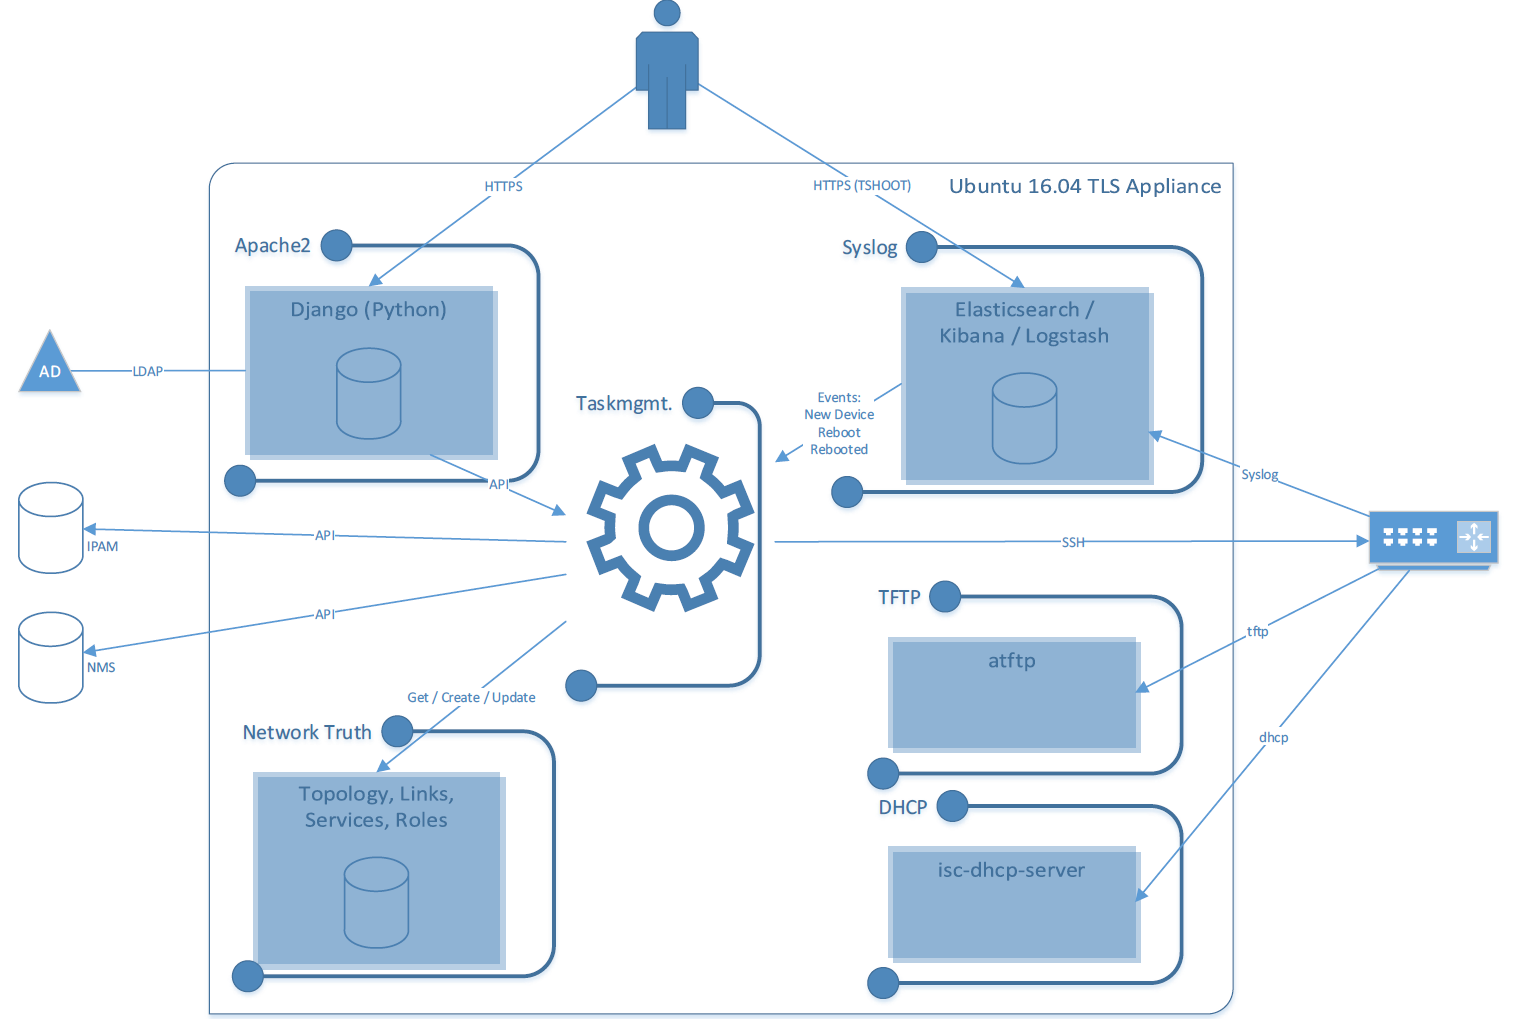
\includegraphics[height = 0.78\textheight]{images/staging_robot_arch01_SwiNOG31.png}
    \caption{\footnotesize Source: SwiNOG \#31 Network Automation – Road trip to an automated Network}
  \end{figure}
\end{frame}

\note{Spend some time to explain the architecture.
  Would I do it again the same?
  With my skills now; Probalby FaaS.
  Django was the right decision. Task management we gambled and lost. More to it soon}

\begin{frame}{Event Based}
  % Explain the idea and workflow. Diagram
  \begin{vfilleditems}
    \item No need to know in advance:
    \begin{vfilleditems}
      \item Serial Number
      \item MAC Address
      \item Model ID
    \end{vfilleditems}
    \item Support for different staging areas
    \item Staging directly at the destination
  \end{vfilleditems}
\end{frame}

\note{Explain the idea of event-based, automatic device discovery, device asking for information. In the end, only one staging area was used.}

\begin{frame}{EEM}
  % L2 does not support EEM, Use TCL
  Disclamer: Needed support for IOS 12 (no Python, no PnP)
  \begin{vfilleditems}
    \item The First idea was to use EEM
    \item EEM is not supported on L2 devices
    \item TCL works on all platforms
    \item TCL has slightly different versions and different libraries
  \end{vfilleditems}
\end{frame}

\note{Disclamer: Needed support for IOS 12 (no Python, no PnP)
  PoC with EEM applets;  figure out that EEM is only available on L3 devices. Finding out that TCL shell also works on L2.
}

\begin{frame}{TCL}
  % Show complexity, How many ifs

  \begin{vfilleditems}
    \item More than 900 lines of code
    \item Around 100 ''if'' statements
    \item Aproxamitly 50 cold showers
  \end{vfilleditems}

\end{frame}

\note{Using TCL was not the best idea I had. It ended up being complex as there are so many ways how to upgrade from one version to the next over the years.
  It has so many if's we can call it already AI as it simulates human behavior upgrading a box.
  The script collects PID, Version, CDP neighbors and talks to hour own API to ask if a job exists.
  If a job exists and the version is not correct the software is updated,
  Config stored in startup and some special Layer 2 commands are executed as some platforms did not configure it correctly at boot time}

\begin{frame}{How it looked - Job Overview}

  \begin{figure}
    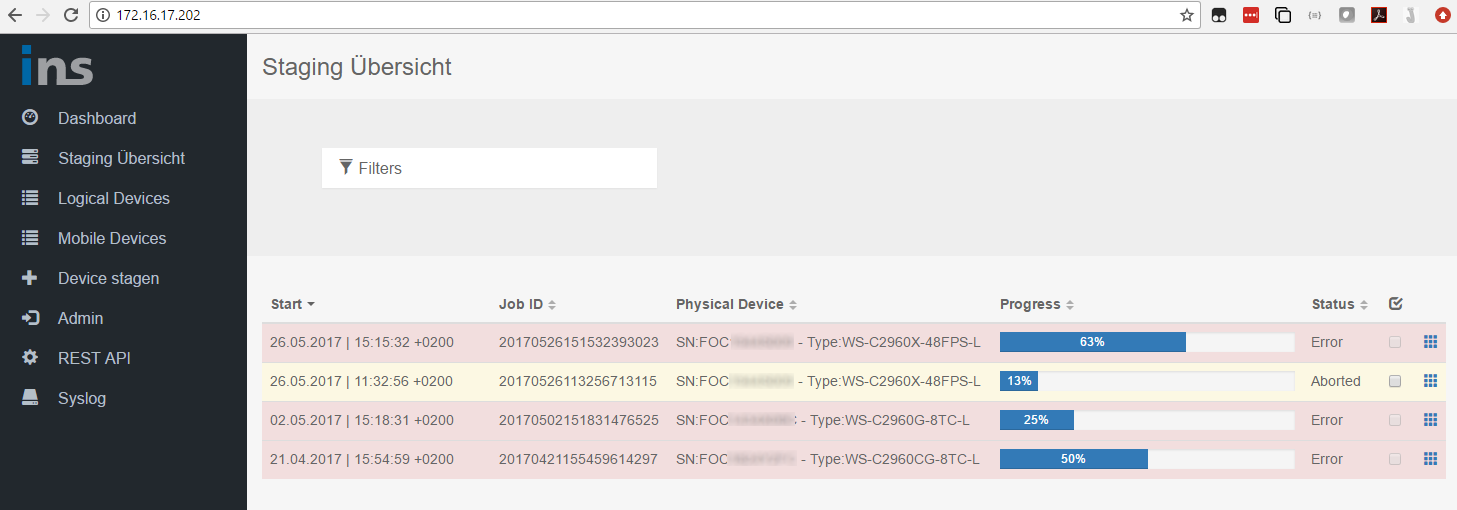
\includegraphics[width = 1.0\textwidth]{images/staging_robot_joblist_SwiNOG31.png}
    \caption{\footnotesize Source: SwiNOG \#31 Network Automation – Road trip to an automated Network}
  \end{figure}

\end{frame}

\note{Don't spend too much time. Django backend rendered with Angular. Okay enough for the time}

\begin{frame}{How it looked - Job Details}

  \begin{figure}
    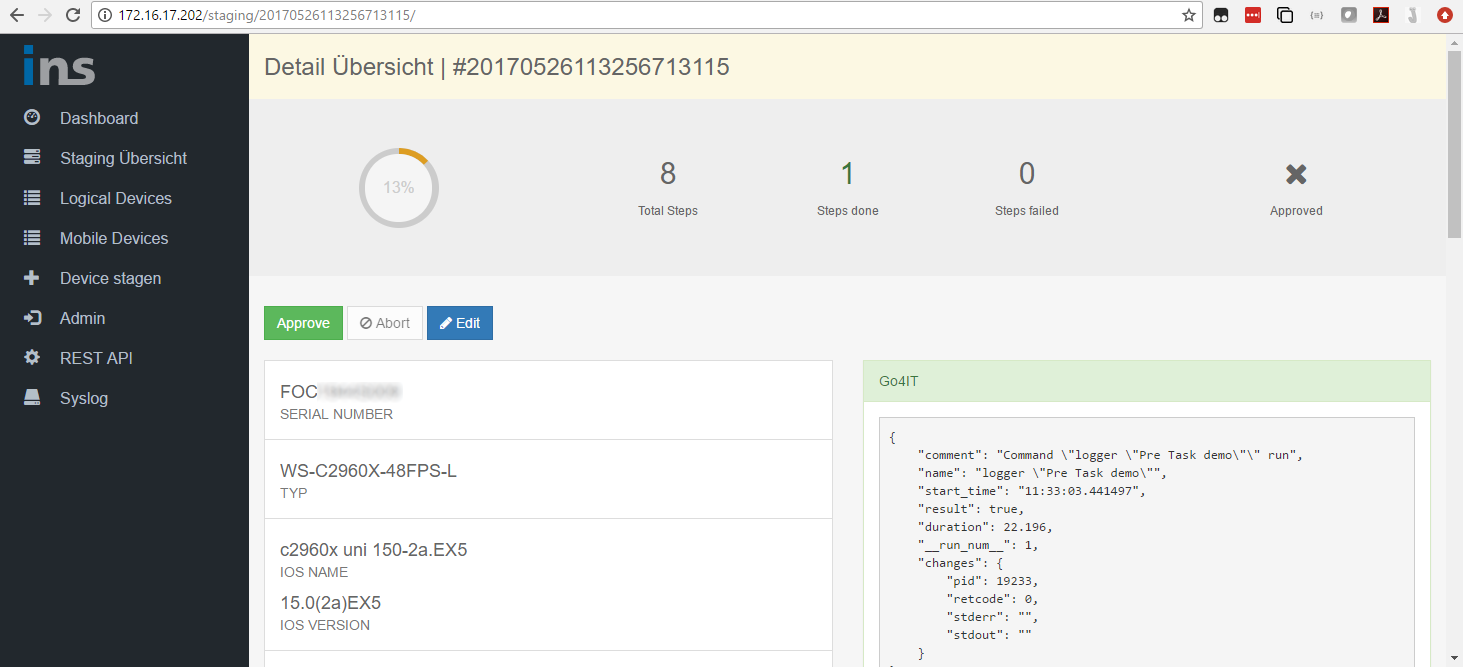
\includegraphics[height = 0.78\textheight]{images/staging_robot_job_SwiNOG31.png}
    \caption{\footnotesize Source: SwiNOG \#31 Network Automation – Road trip to an automated Network}
  \end{figure}

\end{frame}

\note{Don't spend too much time. Point out the task steps are taken out of Salt and the ''ugly'' value is the Salt internal data structure.
  Make sure to have good transparency and make your life easier by allowing the user to troubleshoot}

\begin{frame}[fragile]{SaltStack}
  % Explain why I would not use it anymore
  % show label print step

  %\begin{columns}
  %\begin{column}{0.4\textwidth}
  \begin{vfilleditems}
    \item Using event bus
    \item Provides API
    \item Over time way too many workarounds
  \end{vfilleditems}
  %\end{column}
  %\begin{column}{0.6\textwidth}
  \begin{minted}[fontsize=\footnotesize]{sls}


label_print:
  cmd.run:
    - description: Print label
    - name: print_label.py {{ printer_ip }} 1 "{{ salt['pillar.get']('hostname','') }}"

          \end{minted}
  %\end{column}
  %\end{columns}

\end{frame}

\note{Explain why SaltStack was in the end not a good idea and added dependencies and was hard to make it work. Usage of Salt how it was not intended.}

\begin{frame}{Awesome Features}
  % Hierarchical Network Domain variables
  % Generate WebForm from Template
  % ...
  \begin{vfilleditems}
    \item Hierarchical Network-Domain variables
    \item Generate WebForm from Template variables
    \item Prepare Device Management with SaltStack
    \item Templates and template snippets
  \end{vfilleditems}

\end{frame}

\note{Many great features were implemented because the idea was the user will use it. Be careful to not end up with dead code in the code base.
  All these features are still in the code but not in use (anymore)}

\begin{frame}{Generate Form from Template}

  \begin{figure}
    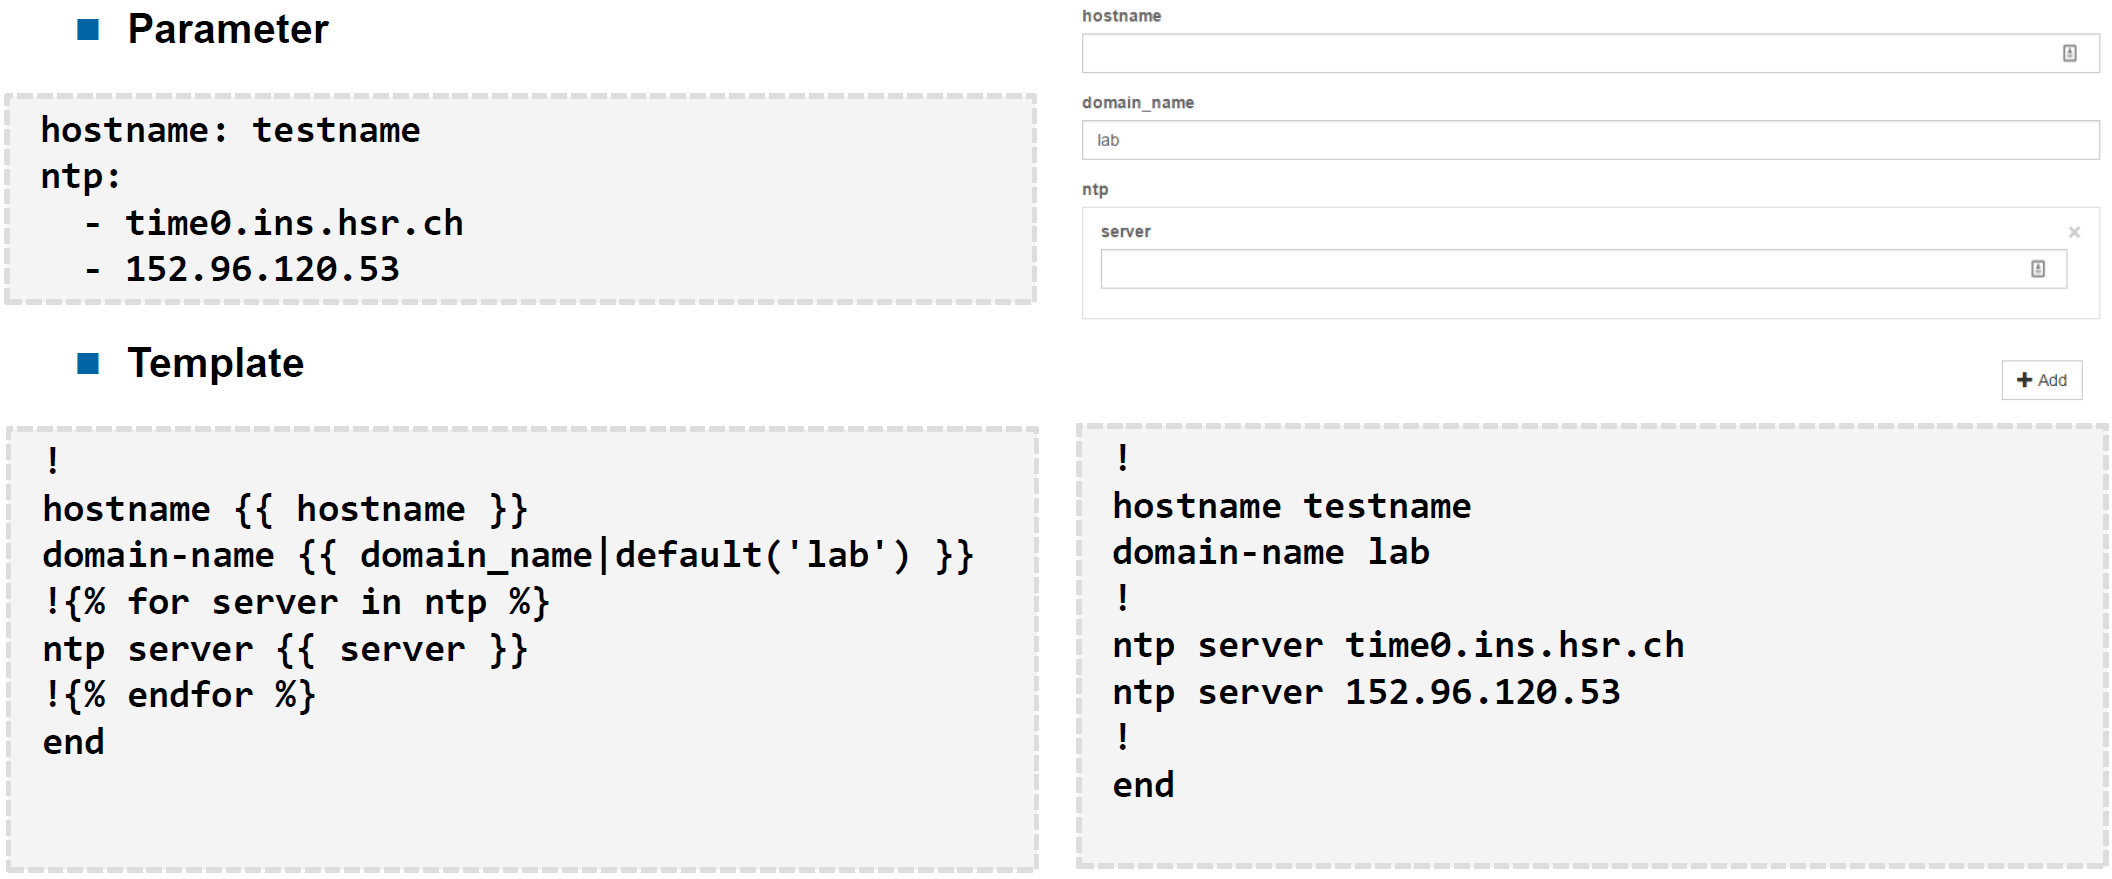
\includegraphics[height = 0.7\textheight]{images/staging_robot_form_generation_SwiNOG31.png}
    \caption{\footnotesize Source: SwiNOG \#31 Network Automation – Road trip to an automated Network}
  \end{figure}

\end{frame}

\note{Was one of my favorite features. Depending on what variables are defined a form was created with list and dict support as well as default value support.
  Was not used and is dead code with dependencies to libraries now. Yes, I should have removed it again from the code base.}

\begin{frame}{''Emergency'' OS upgrade}
  We hit a dot1x bug and need to upgrade 5000 switches ASAP. \\ Could the ''Staging Robot'' do that?
  \begin{flushright}
    \underline{Customer A} (2017)
  \end{flushright}

  \begin{itemize}
    \item Own implementation of Plug\&Play
    \item UI with CSV export/import to select a time window
    \item Slow start
  \end{itemize}
\end{frame}

\note{Wanted to make a simple netmiko script but Customer A convinced me to generate a WebApp to select what time the device is allowed to automatically upgrade it self.
  Was completely integrated into the ''Staging Robot'' afterward but never completely fit into the architecture as some stuff was done quick quick and it worked so why refactor?
  The backend code is still there but not in the frontend anymore as it is not used anymore.}


\begin{frame}{Redesing UI}

  \begin{vfilleditems}
    \item Use synergies from other internally developed tools
    \item SinglePage with react
    \item Integrate multiple backends in the same UI
  \end{vfilleditems}

\end{frame}

\note{Simple UI had its limitations. Frontend engineers created react single page UI trying to use the same for different tools from other internal teams.
  Nice UI but also much more complicated to change something. After some internal restructuring,
  this team does not exist anymore and my react skills are weaker than my sales skills.}

\begin{frame}{Customer B}

  We have a huge rollout upcoming. Could your tool be adapted?
  \begin{flushright}
    \underline{Customer B} (2019)
  \end{flushright}

\end{frame}

\note{New customer wants the same but different. How to avoid having different code bases? It is important to have a plan and keep customers in the loop.
  Workflow on top of staging was needed as the staging was just a part. Could we have avoided it with a better architecture at the beginning?
  Difficult choice between adding unneeded complexity in the beginning and thinking about the future.}


\begin{frame}{Architecture}

  % https://excalidraw.com/#json=S7EEmlCgKVvh3Ombo-oxP,59CqaU7ubo5Bgl90OKOIbA
  \begin{figure}
    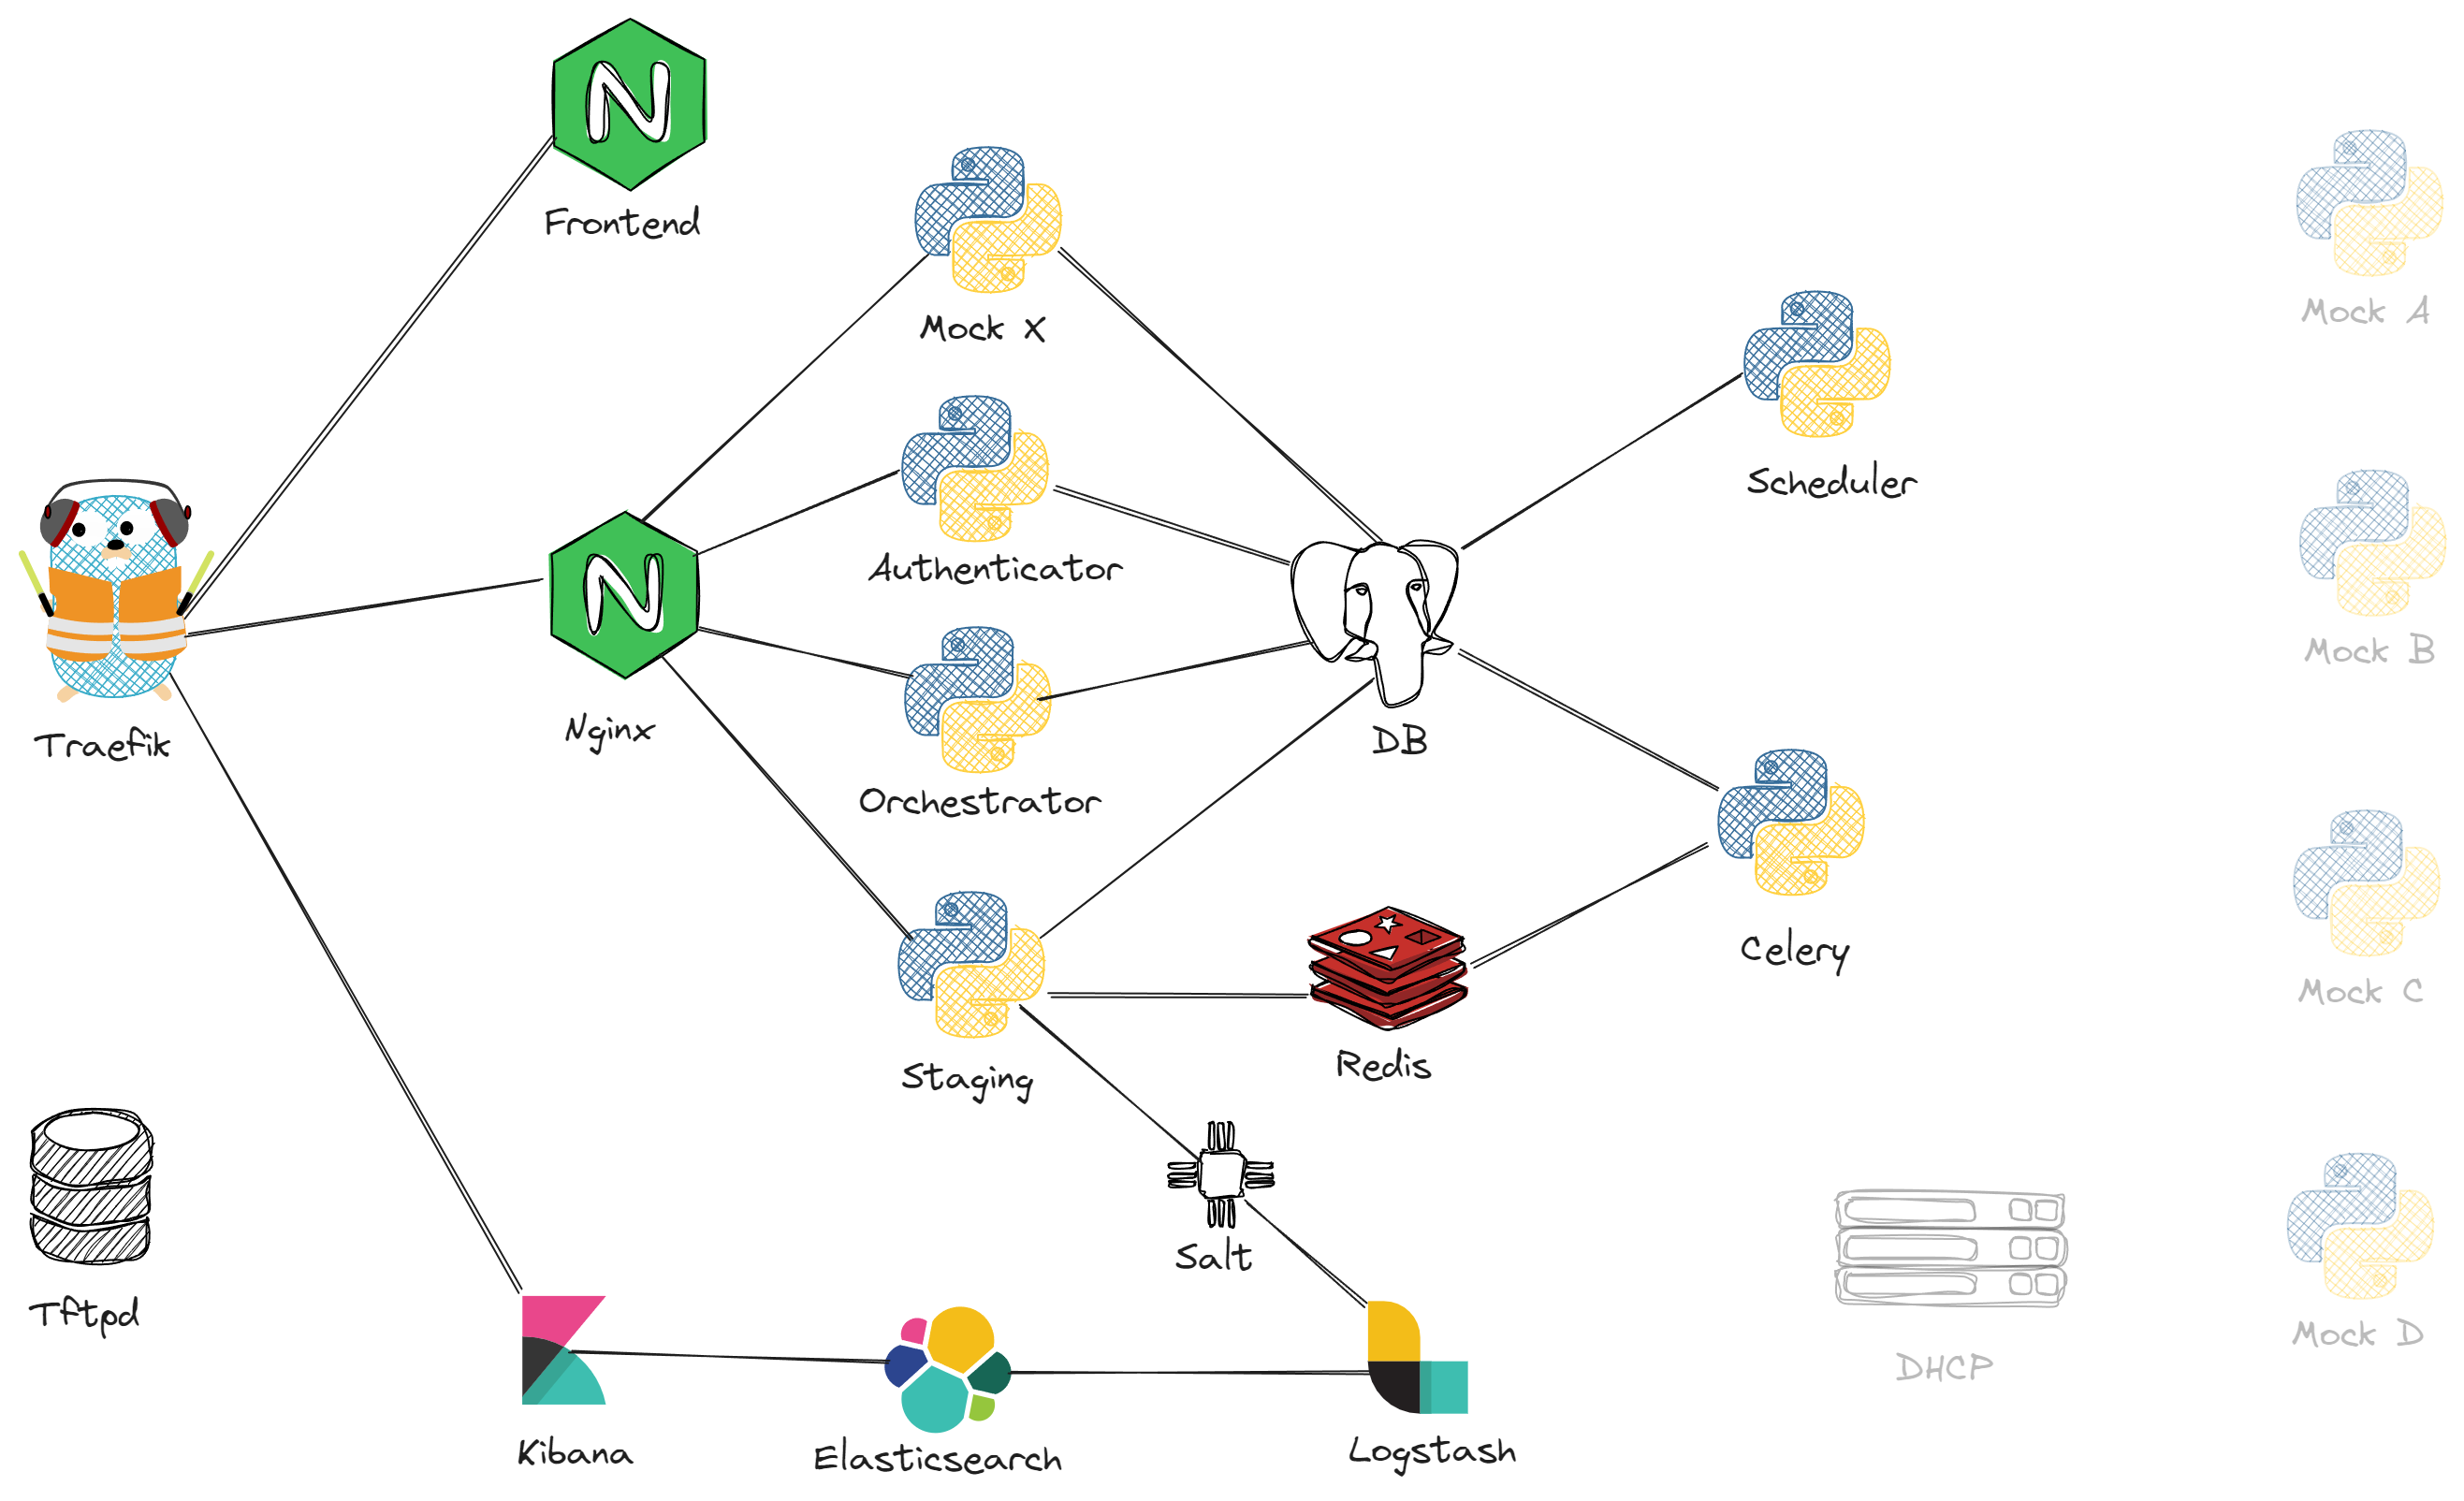
\includegraphics[height = 0.8\textheight]{images/architecture.png}
  \end{figure}

\end{frame}

\note{Here I want to give an overview of the new architecture and how the 17 containers work together.
  We created some mock services because some 3 party tools were not ready and surprised: after more than 4 years one of the mock is still used.
}

\begin{frame}{Addons}

  \begin{itemize}
    \item 1:1 Replace Device
    \item Replacement with a new device
    \item Replace with Stack
    \item Provision/Deprovison Access port (API triggered from ordering system)
    \item ToDo \dots
  \end{itemize}

\end{frame}

\note{Explain shortly the use cases customer B addresses with this solution}

\begin{frame}{Orchestrator}

  \begin{figure}
    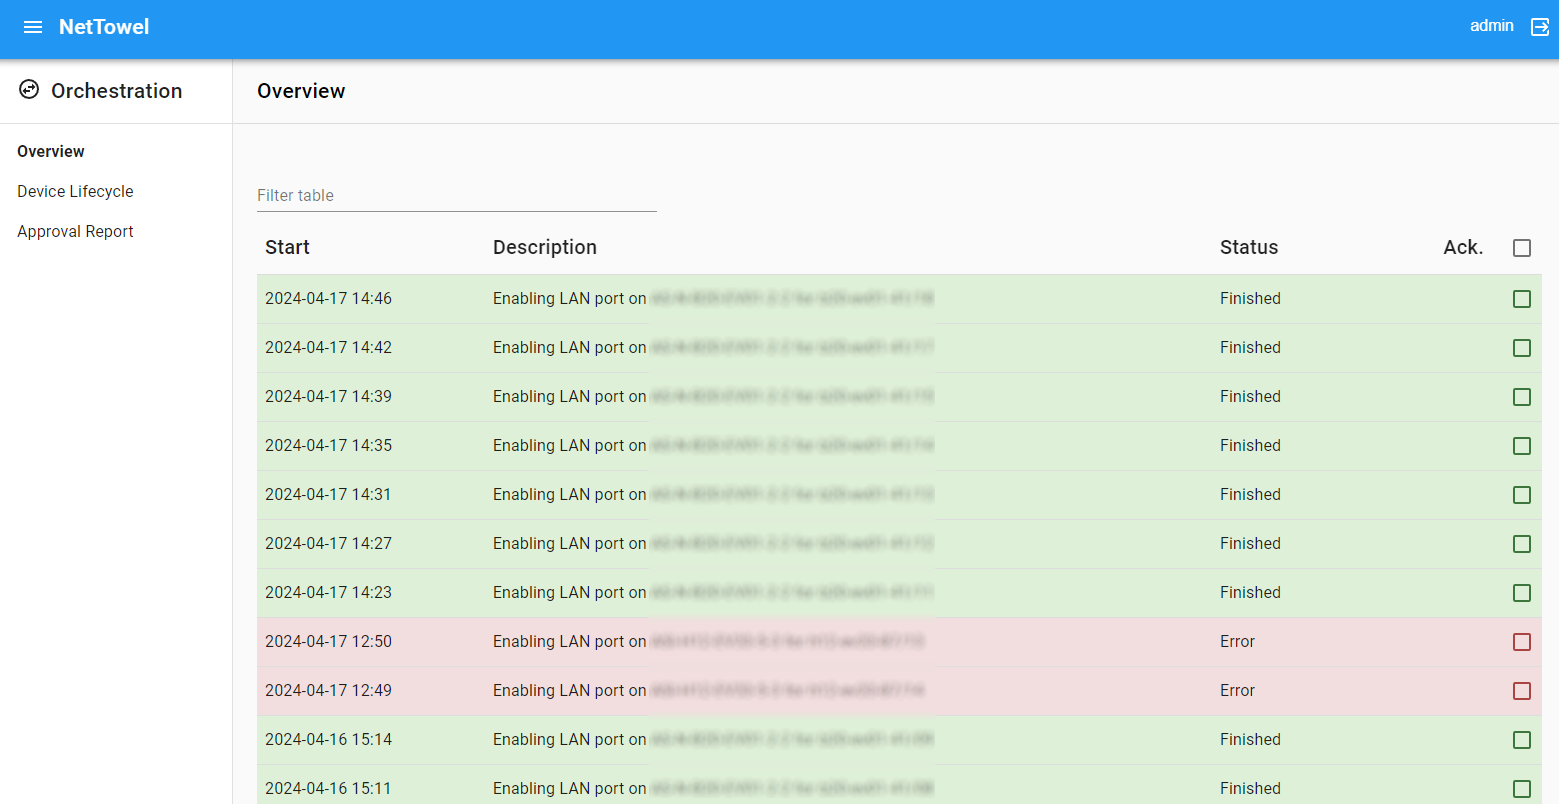
\includegraphics[height = 0.8\textheight]{images/nettowel_orchestration_overview.png}
  \end{figure}

\end{frame}

\note{very quick. how it looks now. One SinglePage to manage the different components}


\begin{frame}{Orchestrator}

  \begin{figure}
    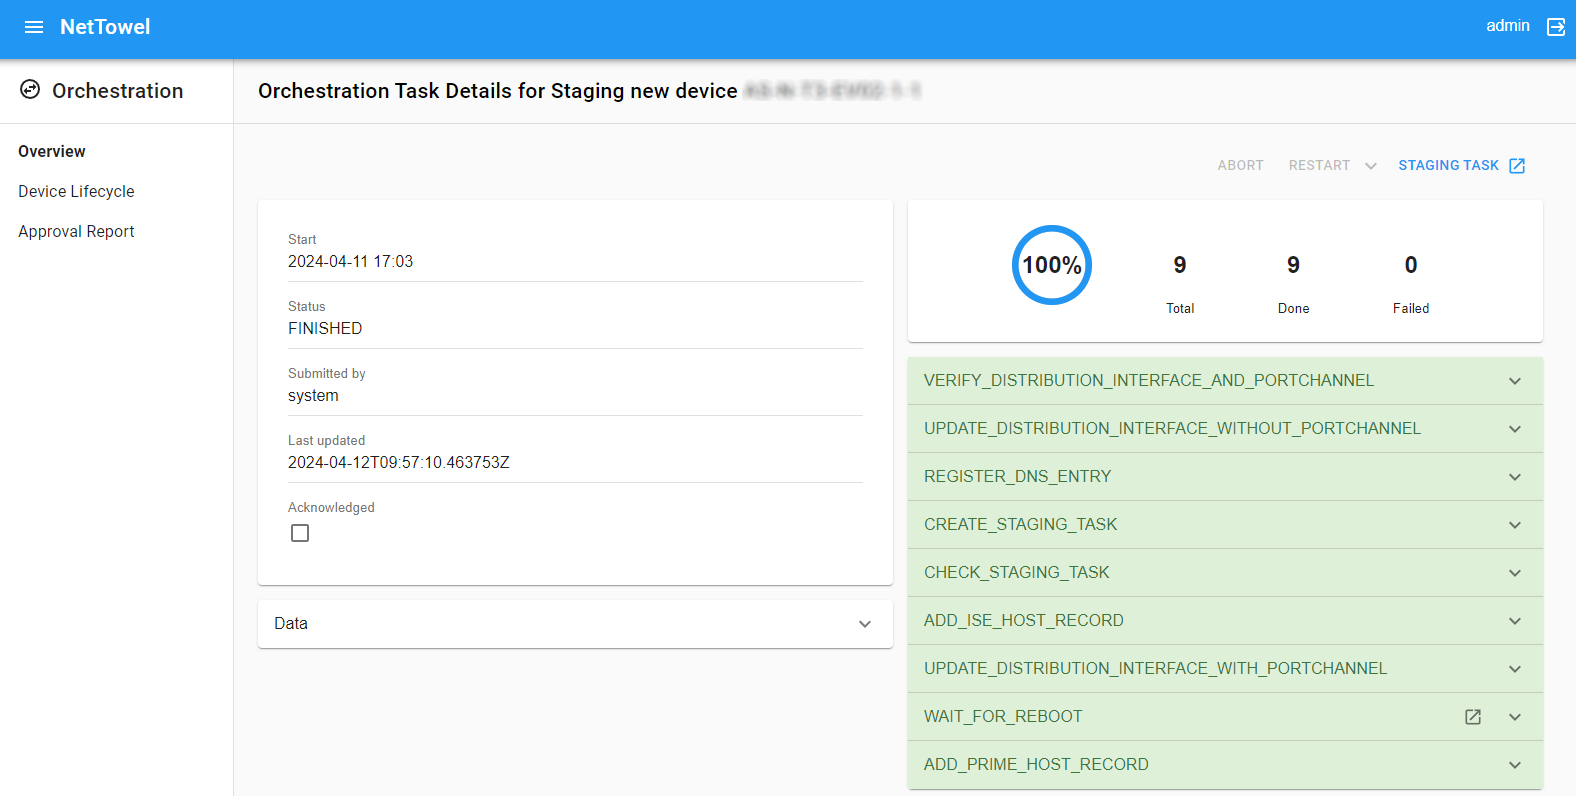
\includegraphics[height = 0.8\textheight]{images/nettowel_orchestration_new_device.png}
  \end{figure}

\end{frame}

\note{very quick}

\begin{frame}{DiY or not?}

  \begin{vfilleditems}
    \item Exactly what you need vs general
    \item Resource-intensive vs locking
    \item Dependencies
    \item ToDo \dots
  \end{vfilleditems}

\end{frame}

\note{At this time I was in another internal team but still the main know-how owner and product owner. We had long discussions about using an existing workflow engine or not.
  The software engineering team ended up implementing a simple workflow engine by themeselves.
  Nice Object-oriented solution. Drawback: only a software developer can extend it. Would a normal do it? Not sure. I was wrong by Salt so maybe I am wrong here too?}


\begin{frame}{Configuration Task}

  \begin{figure}
    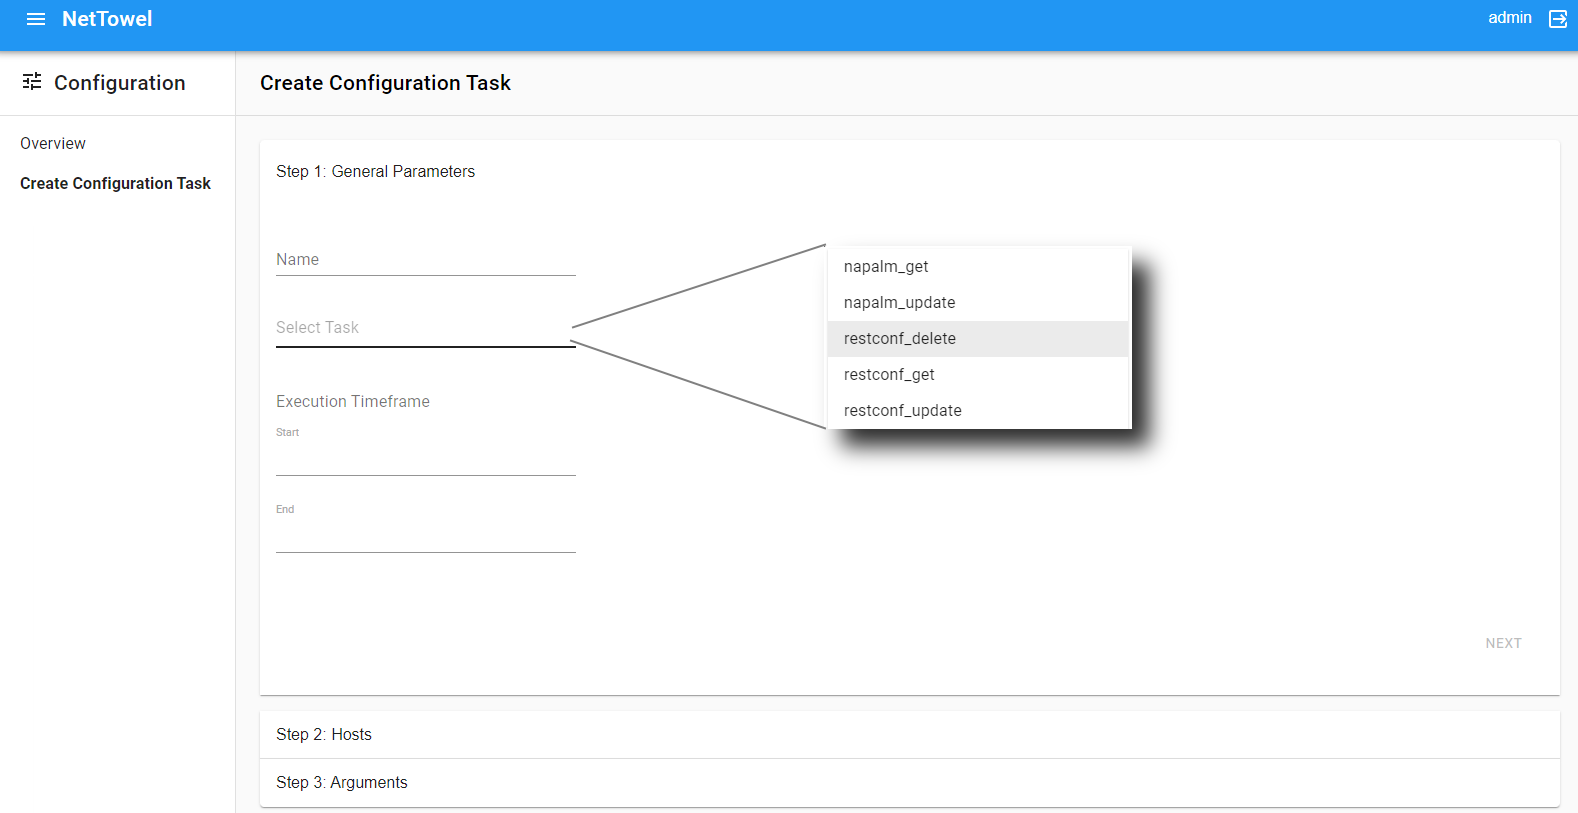
\includegraphics[height = 0.8\textheight]{images/nettowel_config_create_task.png}
  \end{figure}

\end{frame}

\note{Quickly: Added a simple component to abstract some stuff and dependencies and we could scale. }

\begin{frame}{Staging}

  \begin{figure}
    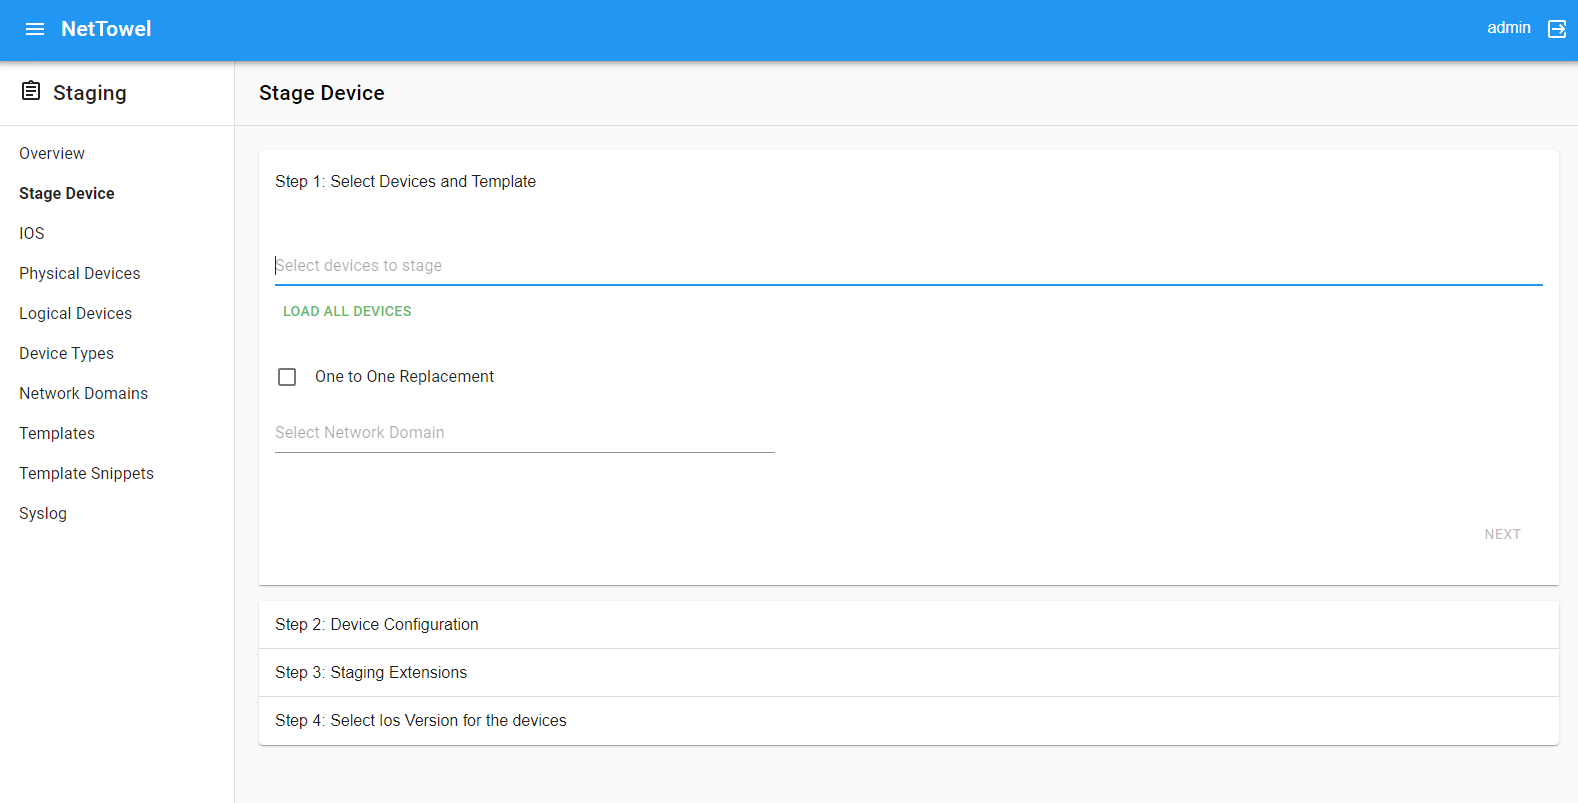
\includegraphics[height = 0.8\textheight]{images/nettowel_staging_new.png}
  \end{figure}

\end{frame}

\note{Wher is the ''Staging Robot''? Still here, still accessible but only used for trouble-shooting and visibility as the staging tasks are created by the orchestration component.}


\begin{frame}{Some numbers}

  Customer A
  \begin{itemize}
    \item Used the Staging Robot until mid-2023
    \item Staged around 9'000 L2/L3 devices
    \item Around 5'000 PnP OS Upgrades
  \end{itemize}

  Customer B
  \begin{itemize}
    \item In production
    \item Todo: \dots
    \item Todo: \dots
  \end{itemize}


\end{frame}

\note{Some numbers to show the dimensions. The TCL script is quite stable xD.
  ToDo: I need to get info from customer B}


\begin{frame}{Using Open Source}

  \begin{vfilleditems}
    \item Be prepared to debug the code
    \item Avoid basing on forks
    \item Try to be up to date
    \item ToDo \dots
  \end{vfilleditems}

\end{frame}

\note{Need to work on this but want to point out what it means to rely on open-source tools. I made many PR and fixes in the last 9 years.}

\begin{frame}{Key Points}

  \begin{vfilleditems}
    \item Don't be afraid of failing
    \item Do not over-engineer
    \item Who can maintain this in 5 years?
    \item Does the customer need this feature or do you want it?
    \item No shortcuts
  \end{vfilleditems}

\end{frame}

\note{This is also not final yet. Want to have some more meat.}

\end{document}